\documentclass[UTF8]{article}
\usepackage{graphicx}
\usepackage{CJK}
\usepackage{epstopdf}
\usepackage{float}
\usepackage{subfig}
\usepackage{geometry}
\geometry{left=1.7cm,right=1.7cm,top=2.0cm,bottom=2.0cm}
\begin{document}
\begin{CJK}{UTF8}{gkai}
\title{数字信号处理实验报告}
\author{杨庆龙\quad 1500012956\\yangqinglong@pku.edu.cn}
\date{2018.6}
\maketitle

\section{实验原理}
\subsection{原理框图}
\begin{figure}[H]
    \centering
    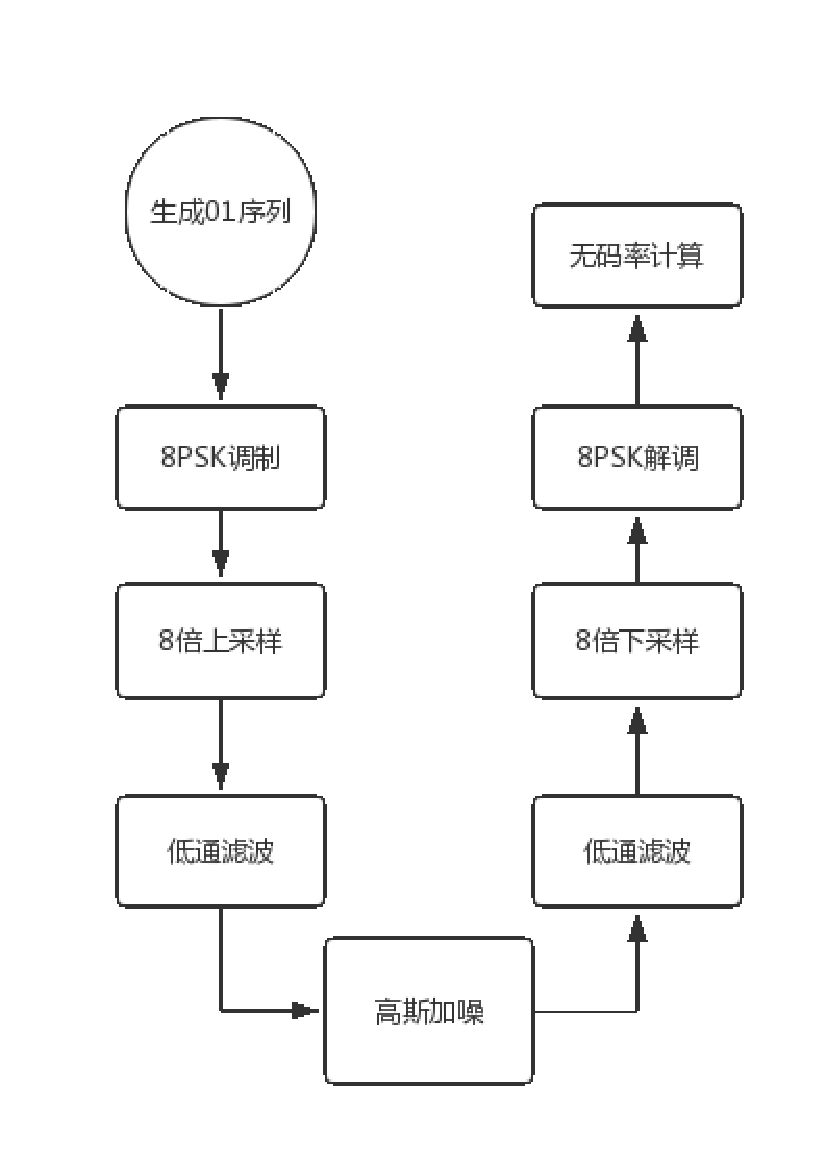
\includegraphics[scale=0.5]{block.eps}
    \caption{实验原理图}
    \label{blocks}
\end{figure}
\subsection{生成随机10序列(get\_bits.m)}
由于matlab中的rand函数只能生成0到1的随机数,但我们需要的是01序列,所以考虑先将随机的浮点数扩大256倍,取整取余后即可得到随机01序列.
\subsection{8PSK调制}
\subsubsection{二进制转八进制(bit2oct.m)}
由于8PSK中的一个符号代表三个比特,所以可以先将二进制序列转为八进制序列以方便后续运算.
\subsubsection{相位调制}
此处假设,信号传输速率为3k\ symbol/s,传输一个symbol需要载波的一个完整周期,则信号带宽约为6kHz.又由奈奎斯特采样定理得,采样频率至少为12kHz,又由于应当留有适当的余量,所以此处选用24kHz的采样率,即一个周期采8个点.\\
因此,依据8PSK调制公式\ref{equ1}$$\label{equ1}A_m=cos(\omega t+\frac{m\pi}{4})$$得到连续时域波形,再使用8倍的采样率采样,即可得到离散的发送信号.
\subsection{八倍上采样}
八倍上采样即在两个信号之间插入7个0即可,使用matlab自带的upsample函数即可
\subsection{低通滤波器设计}
按照调制部分所设计的,采样频率到达24kHz,而信号带宽不变,因此该滤波器参数定为窗函数设计法,凯瑟窗,$F_{s}=24kHz,F_{pass}=6kHz,F_{stop}=8kHz,\delta_a=0.1,\delta_b=80$.
该滤波器的频率响应和单位冲激响应如图
\begin{figure}[H]
  \centering
  \subfloat[滤波器频率响应曲线]{\label{lowpass_mor}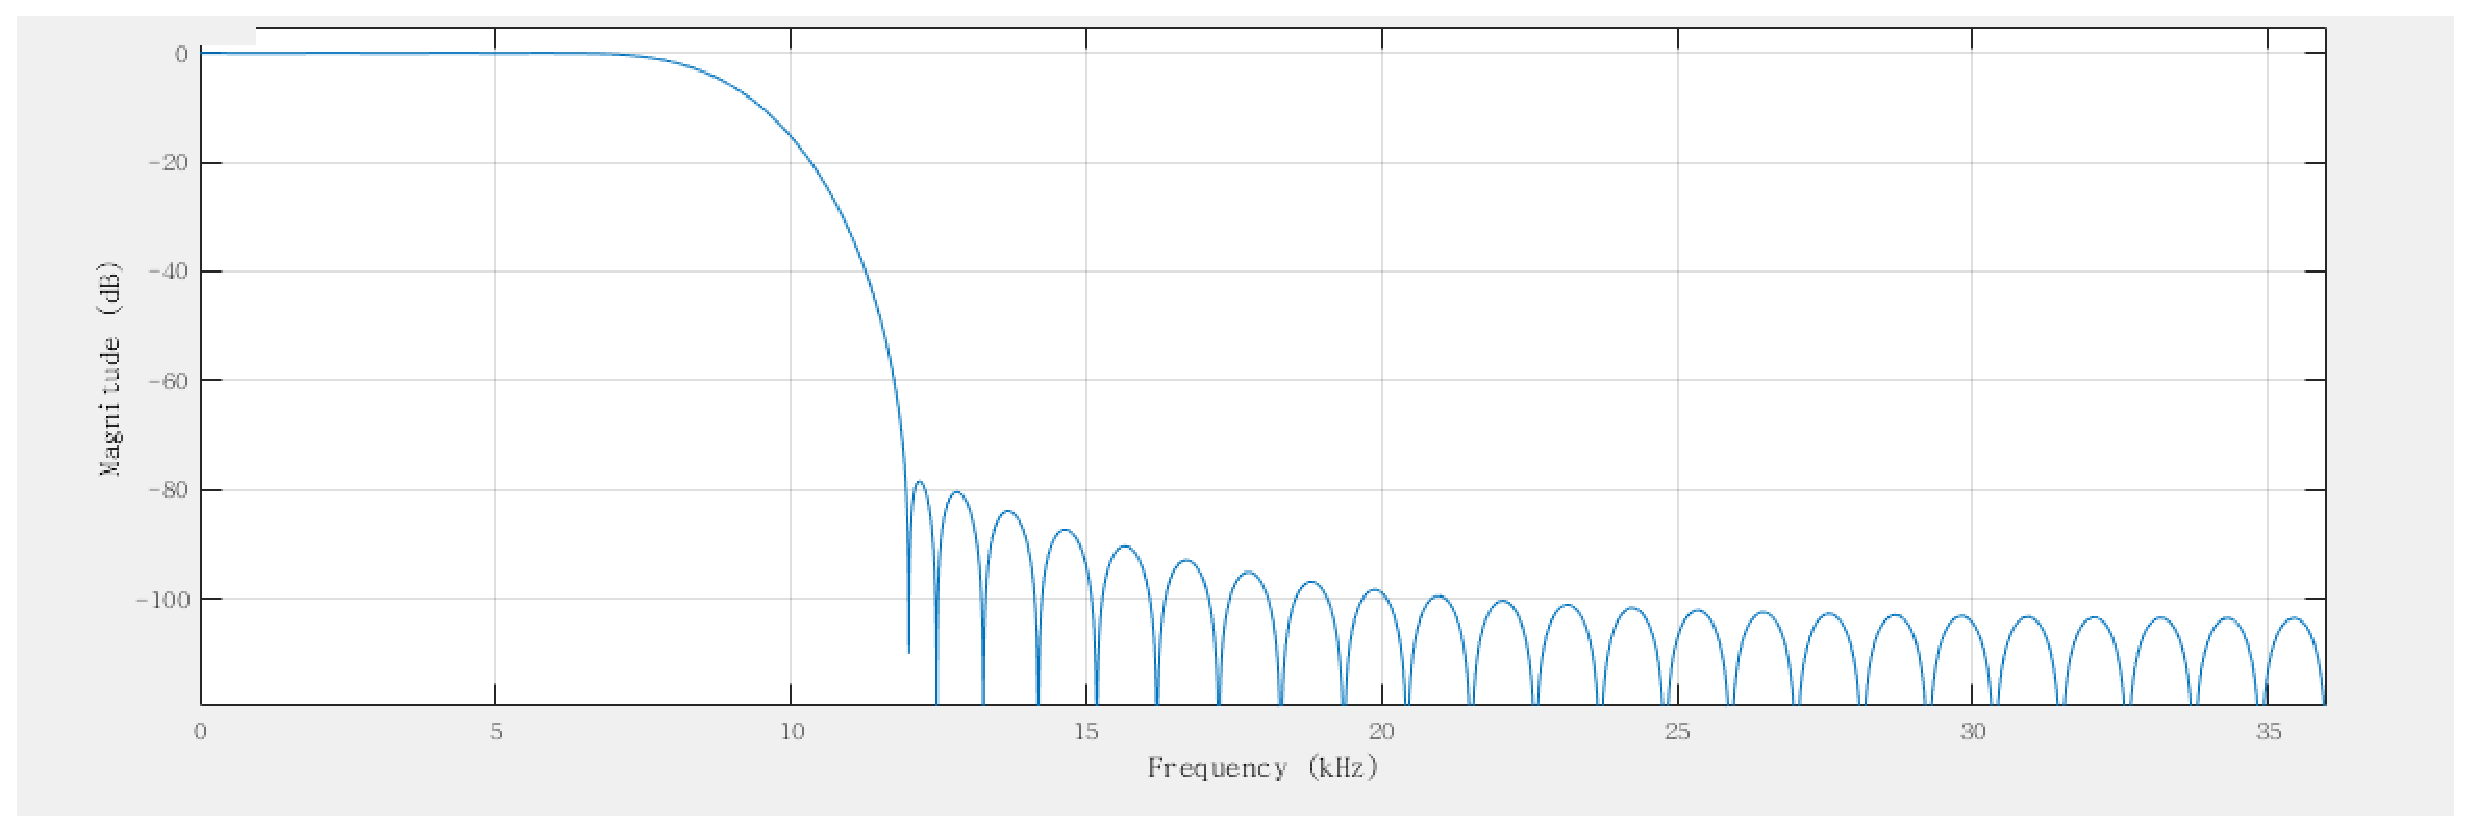
\includegraphics[width=0.5\textwidth]{mor.eps}}
  \subfloat[滤波器单位冲激响应曲线]{\label{lowpass_pulse}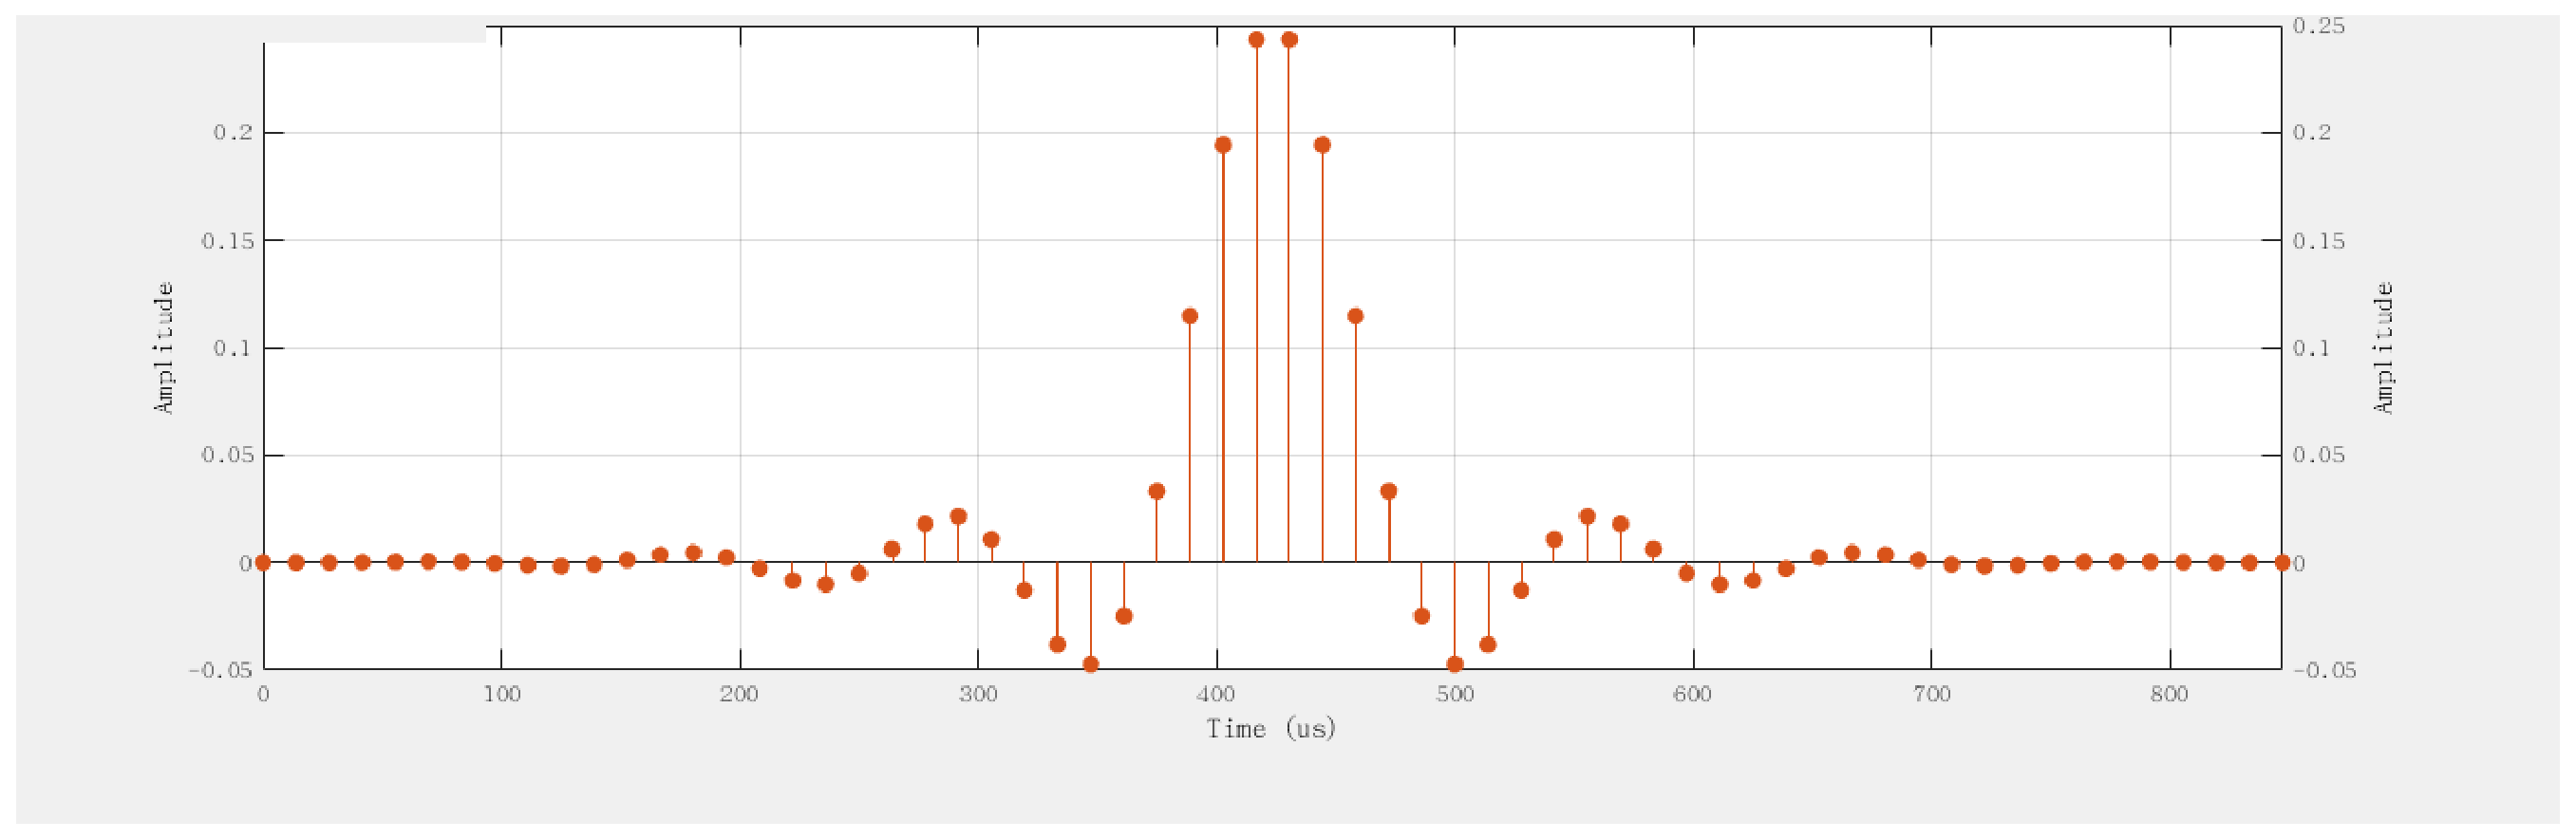
\includegraphics[width=0.5\textwidth]{pulse.eps}}
\end{figure}
\subsection{低通滤波(filting.m)}
使用线性卷积的方法实现滤波,由于滤波存在相位延迟的问题,所以还将卷积结果中的适当长度的头尾去掉.
\subsection{高斯加噪}
为模拟信号通过高斯信道,选用matlab自带的awgn函数作为加噪函数,加噪所用SNR计算公式为
$$SNR=\frac{E_b}{N_0}+10log_10(k)-10log(Nsamp)$$
其中,k为每个符合的比特数
\subsection{八倍下采样}
此处使用matlab自带的downsample函数实现下采样功能
\subsection{8PSK解调}
\subsubsection{相位解调}
使用相干解调的方法实现8PSK解调,依据公式\ref{equ2}和\ref{equ3}
$$\label{equ2}\int cos(\omega t+\phi)cos(\omega t)dt=\frac{sin\phi}{2}$$
$$\label{equ3}\int cos(\omega t+\phi)sin(\omega t)dt=\frac{cos\phi}{2}$$
计算出输入信号在cos和sin方向的分量,进而得到如\ref{stars}所示的星座图,最后依据最大近邻的原则判断输入信号symbol的具体数值.
\begin{figure}[H]
    \centering
    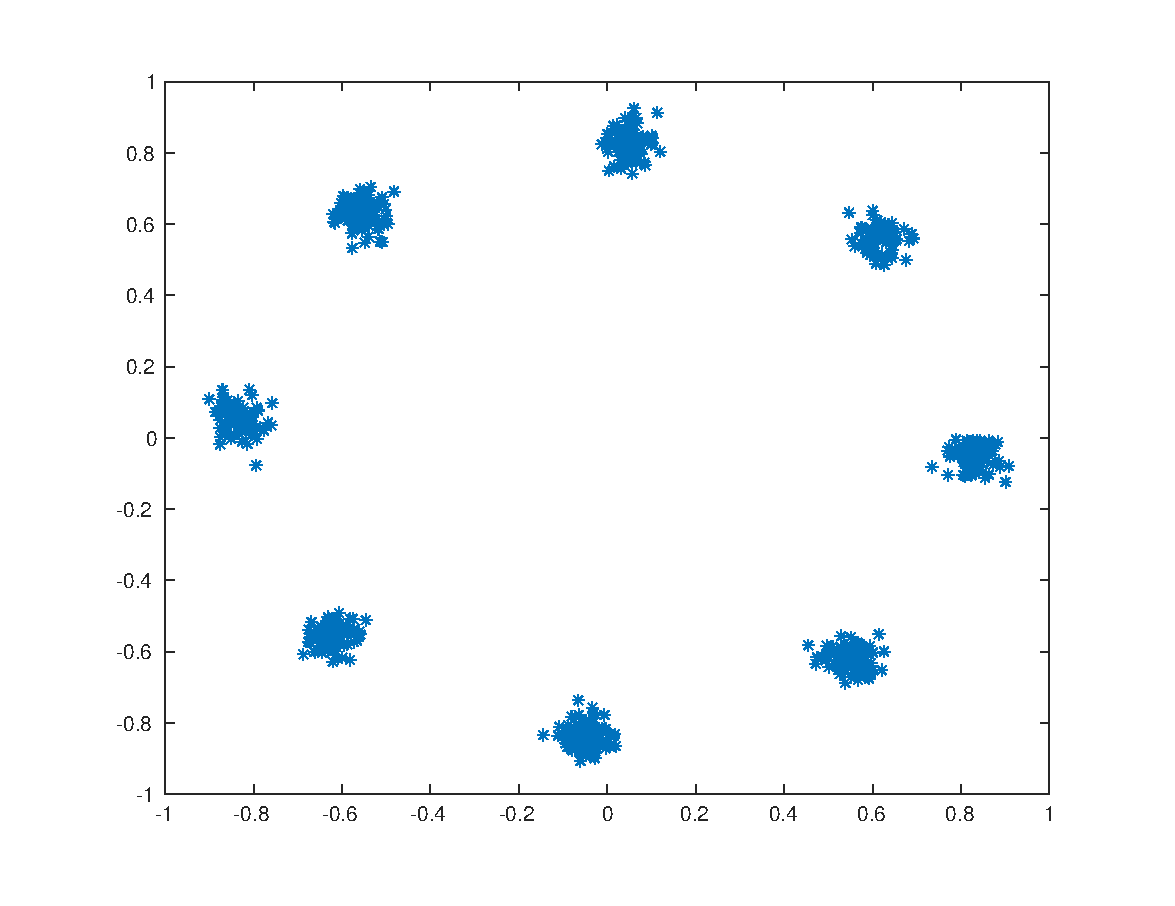
\includegraphics[scale=0.5]{stars.eps}
    \caption{星座图}
    \label{stars}
\end{figure}
\subsubsection{八进制转二进制(oct2bit.m)}
与调制时相对,解调得到的是八进制数,所以还需要转换为二进制数才能进行下一步的处理与比较.
\subsection{误码率计算}
使用原始01序列和解调得到的数据进行比较,用出错比特数比上总比特数即可得到误码率.
$$Ber=\frac{N(error)}{N(all)}$$
\section{实验结果}
为了使时域波形不那么混乱,以下时域波形均为输入60bit时的图像.
\subsection{图1}
\begin{figure}[H]
    \centering
    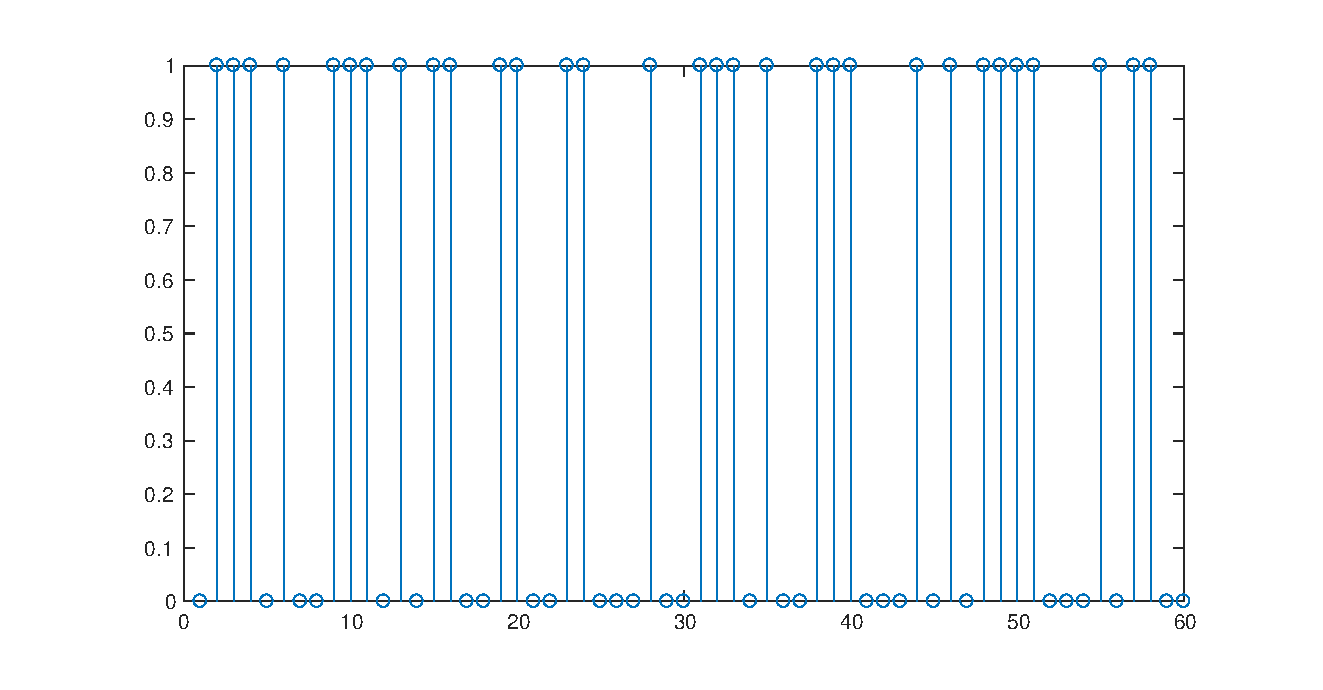
\includegraphics[scale=0.7]{plot1.eps}
    \caption{01序列时域图}
    \label{blocks}
\end{figure}
从图中可以看到,输入数据为0,1随机分布的离散序列.
\subsection{图2}
\begin{figure}[H]
    \centering
    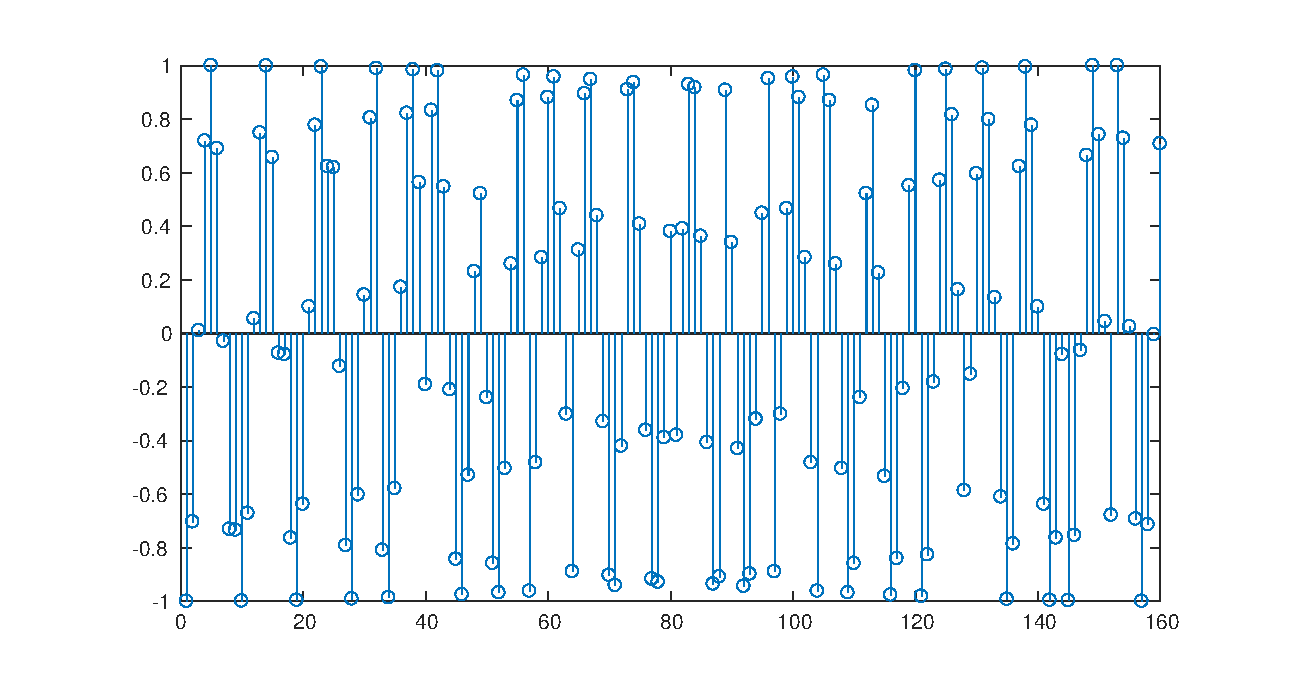
\includegraphics[scale=0.7]{plot2.eps}
    \caption{8PSK调制图像}
    \label{blocks}
\end{figure}
从图中可以看到,调制后的信号波形能在一个周期内为正弦函数的形状特征,但不同周期又有着不一样的相位.
\subsection{图3}
\begin{figure}[H]
    \centering
    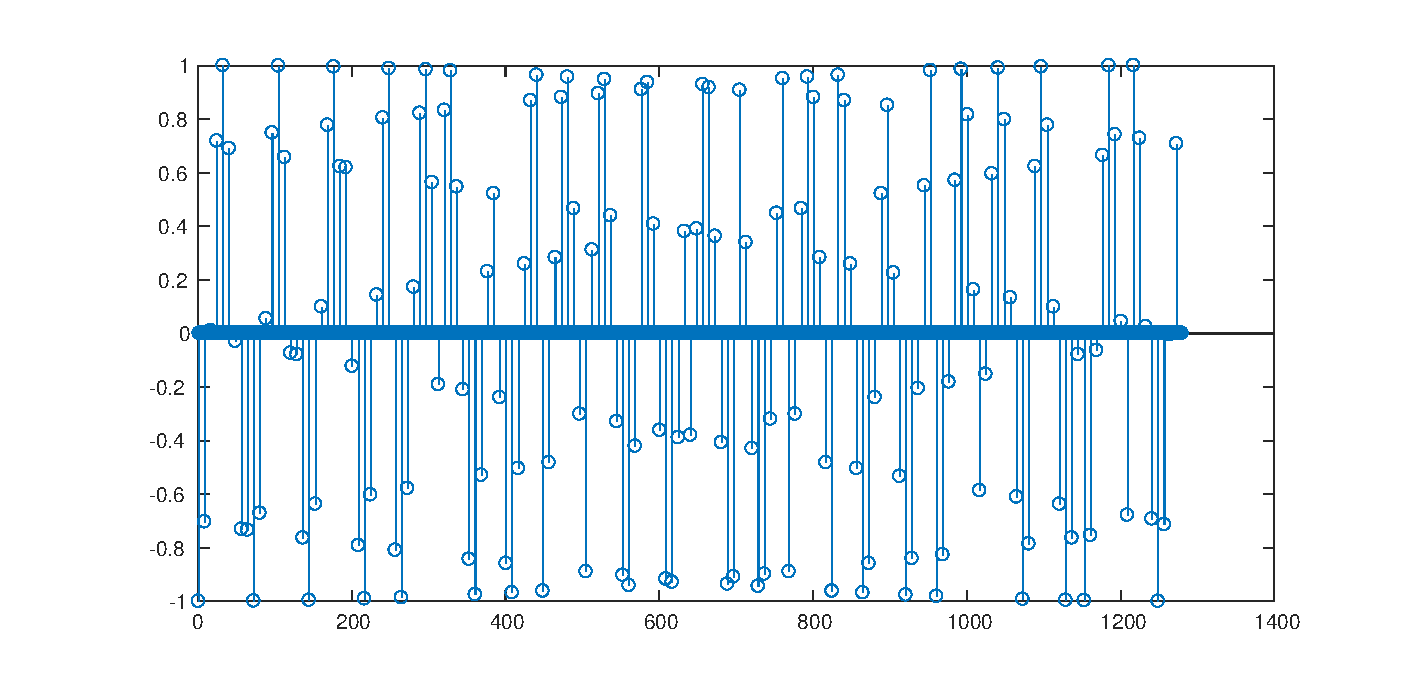
\includegraphics[scale=0.7]{plot3.eps}
    \caption{八倍上采样图}
    \label{blocks}
\end{figure}
从图中可以看到,经过八倍上采样后,在图二的两个值之间插入了7个零.
\subsection{图4}
\begin{figure}[H]
    \centering
    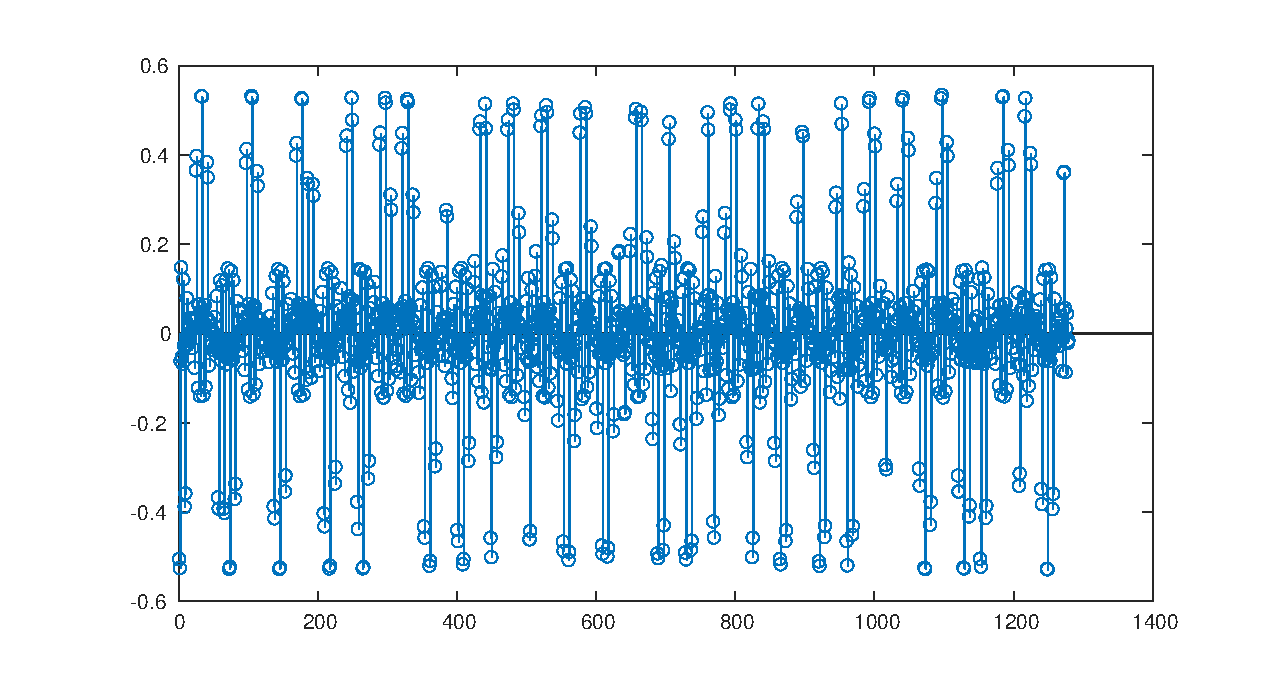
\includegraphics[scale=0.7]{plot4.eps}
    \caption{发送低通滤波图}
    \label{blocks}
\end{figure}
在低通滤波的作用下,原本信号中的突变都变得平滑起来,并在原本为0的地方出现了相应的起伏,即信号中的高频分量被大量滤去,只剩下缓变的低频分量.
\subsection{图5}
\begin{figure}[H]
    \centering
    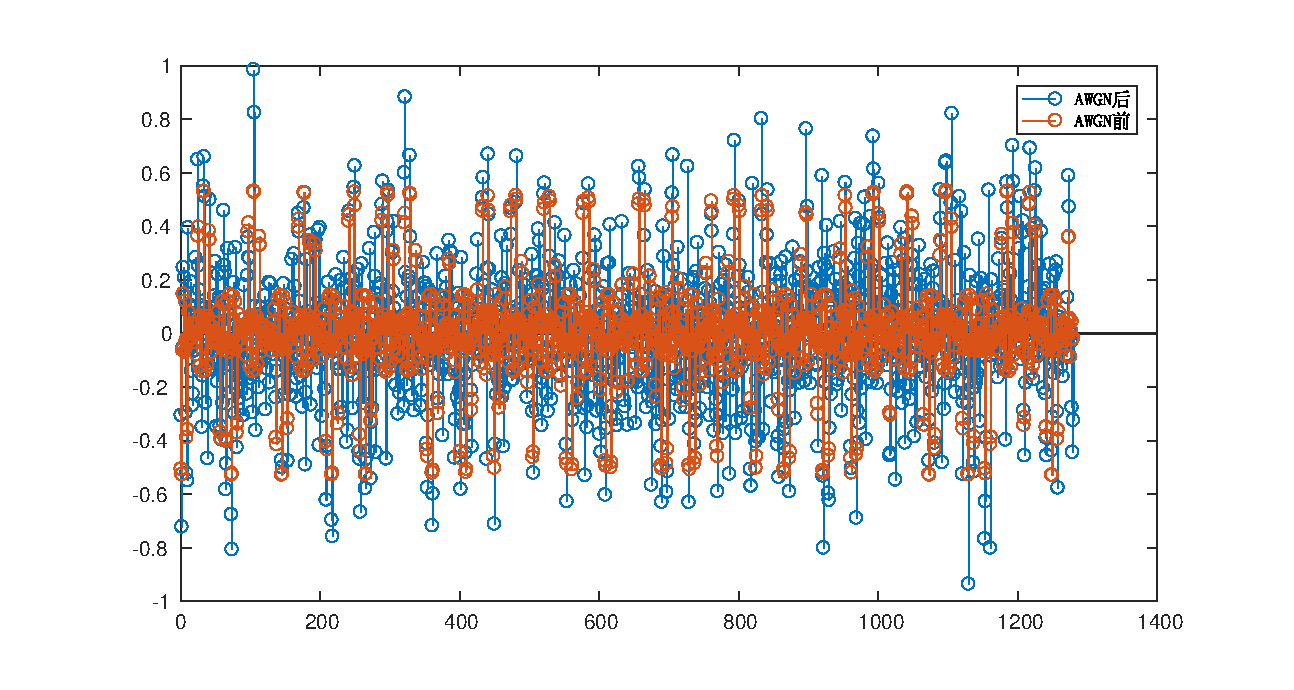
\includegraphics[scale=0.7]{plot5.eps}
    \caption{加噪波形图}
    \label{blocks}
\end{figure}
加噪之后,信号的幅度变化变大,即信号又加入了不少高频分量.
\subsection{图6}
\begin{figure}[H]
    \centering
    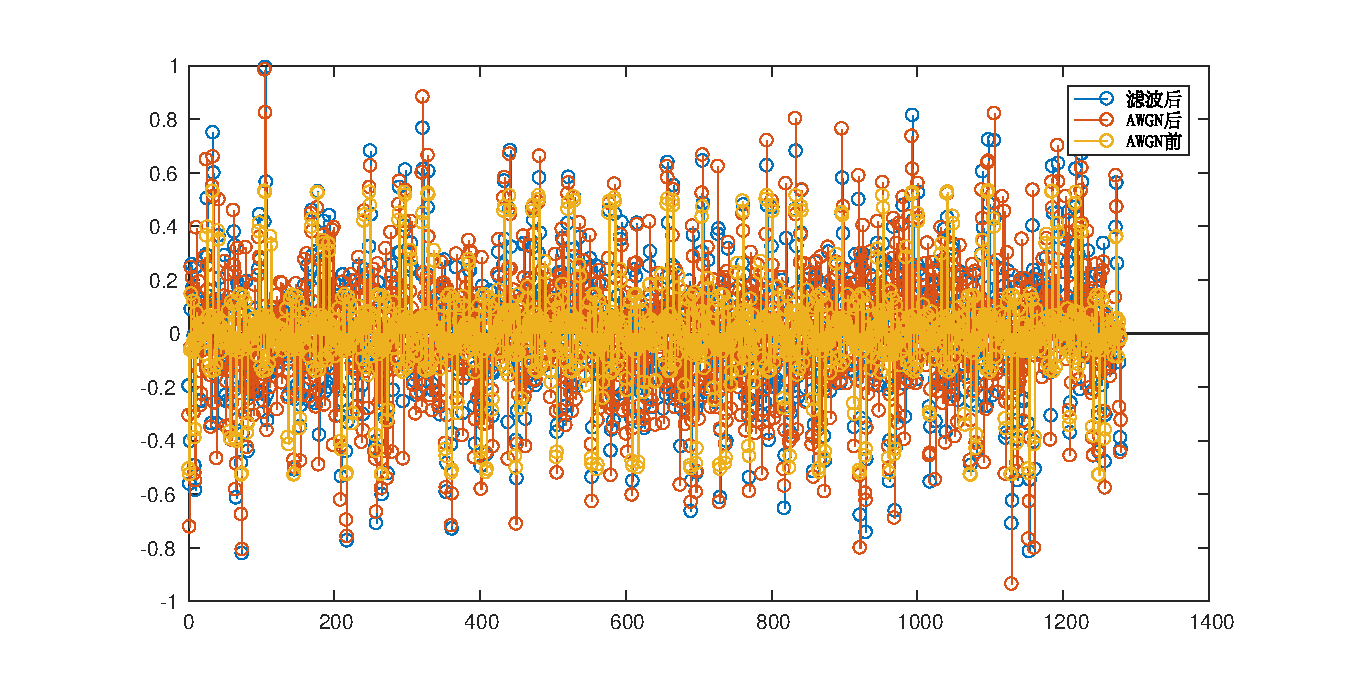
\includegraphics[scale=0.7]{plot6.eps}
    \caption{接收后低通滤波图}
    \label{blocks}
\end{figure}
滤波后,由于高频噪声被去掉,信号又变得平缓了起来.
\subsection{图7}
\begin{figure}[H]
    \centering
    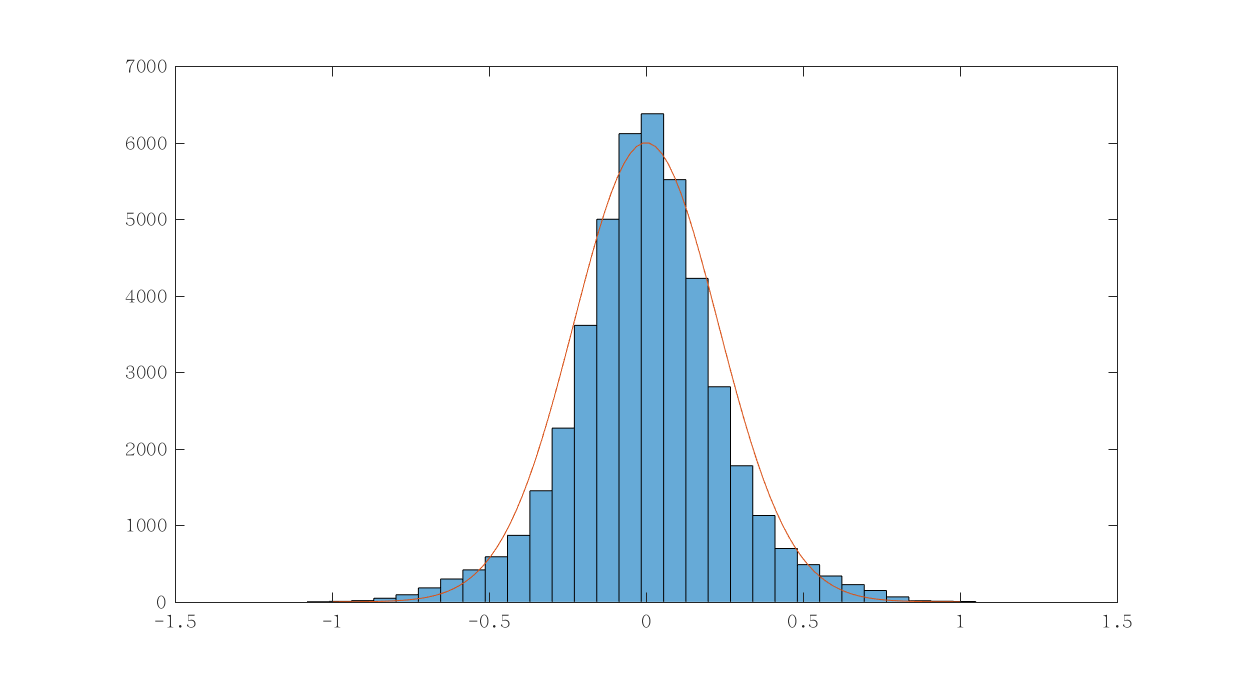
\includegraphics[scale=0.7]{plot7.eps}
    \caption{接收信号PDF图}
    \label{blocks}
\end{figure}
将接收到的信号画成30列的直方图,就能得到该信号的PDF图.由于所加噪声为高斯噪声,所以期望得到的图像应当近似符合高斯分布,而实际所得到的分布与均值为0,方差为0.23的高斯分布符合较好,与期望相符.
\subsection{图8}
\begin{figure}[H]
    \centering
    \includegraphics[scale=0.7]{plot9.eps}
    \caption{bit对比图}
    \label{blocks}
\end{figure}
从bit对比图中可以看到,该传输过程有一定量出错的bit.
\subsection{图9}
\begin{figure}[H]
    \centering
    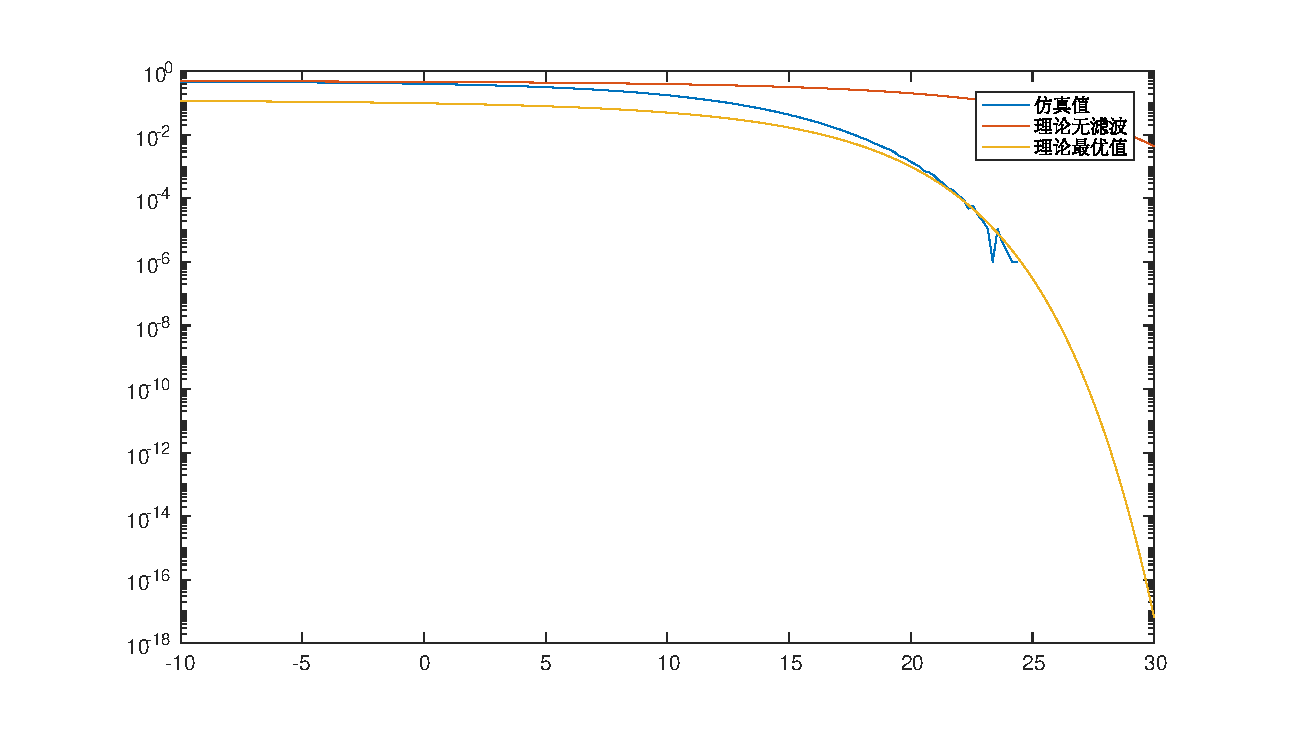
\includegraphics[scale=0.7]{bier.eps}
    \caption{仿真误码率及理论误码率比较}
    \label{blocks}
\end{figure}
在该图中,分别展示出理论无滤波的误码率曲线,理论最优滤波的误码率曲线以及我们仿真得到的误码率曲线.从这三条曲线可以看出,使用低通滤波后,该系统的误码率明显下降,抗噪声能力明显增强.但使用滤波器后在较低信噪比的情况下系统性能与理论最优还是有一定区别,但在较好信噪比的条件下能够接近理论最优值,这说明凯瑟窗具有一定的抗符号间干扰的能力,否则在高信噪比的情况下系统性能应该与理论最优有着明显差异.

\end{CJK}
\end{document}
